% =======================================================================
% =                                                                     =
% =======================================================================
% -----------------------------------------------------------------------
% - Author:     Chaua Queirolo                                          -
% - Version:    001                                                     -
% -----------------------------------------------------------------------
\documentclass[a4paper,11pt]{article}    

% =======================================================================
% PACKAGES
% =======================================================================

% Language support
\usepackage[brazil]{babel}
\usepackage[utf8]{inputenc}
\usepackage[T1]{fontenc}
\usepackage{ae,aecompl}

% Configuration
\usepackage{url}
\usepackage{enumerate}
\usepackage{color}
\usepackage[svgnames,table]{xcolor}
\usepackage[margin=2cm,includefoot]{geometry}

% Tabular
\usepackage{multirow}
\usepackage{multicol}

% Images
\usepackage{graphicx}
\usepackage{caption}
\usepackage[scriptsize]{subfigure}
\usepackage{epstopdf}
\usepackage{float}% http://ctan.org/pkg/{multicol,lipsum,graphicx,float}

% Math
\usepackage{mdwtab}	% bug rowcolor
\usepackage{amssymb}
\usepackage{amsmath}
\usepackage{footnote}

% References
\usepackage[sort,nocompress]{cite}
\usepackage{MnSymbol}
% =======================================================================
% VARIABLES
% =======================================================================

% Space between the lines in a table
\renewcommand{\arraystretch}{1.3}

% Define a new column type
\newcolumntype{x}[1]{>{\raggedright\hspace{0pt}}p{#1}}%

% Controle das Margens
\sloppy
\tolerance=9999999

% Espaço entre colunas
\setlength{\columnsep}{.9cm}


% Configuration
\usepackage{lipsum}
\usepackage{blindtext}

% =======================================================================
% HEADER
% =======================================================================

\title{Estudo de métodos e estratégias para detecção de segmentação de faces de pessoas em imagens}
\author{Felipe Lopes\\E-mail: {\tt felipe\_lopes@outlook.com}}
\date{}

\newenvironment{Figure}
  {\par\medskip\noindent\minipage{\linewidth}}
    {\endminipage\par\medskip}

% =======================================================================
% DOCUMENT
% =======================================================================
\begin{document}
\graphicspath{ {imgResumo/} }
\maketitle

\begin{multicols}{2}
\section{Resumo}
A saída da maioria dos sensores consiste de uma forma de onda de tensão contínua cuja amplitude e o comportamento no espaço estão relacionados ao fenômeno físico que está sendo captado pelos sensores. Para criar uma imagem digital, precisamos converter os dados contínuos que foram captados para o formato digital. Isso envolve dois processos: amostragem e quantização.

\subsection{Conceitos básicos de amostragem e da quantização}
Na figura 1, temos uma imagem contínua e queremos converter a mesma para o formato digital. Para converte-la ao formato digital, temos de fazer a amostragem da função em ambas as coordenadas de amplitude. A digitalização dos valores de coordenada é chamada amostragem. A digitalização dos valores de amplitude é chamado de quantização.
\begin{Figure}
	\centering 
	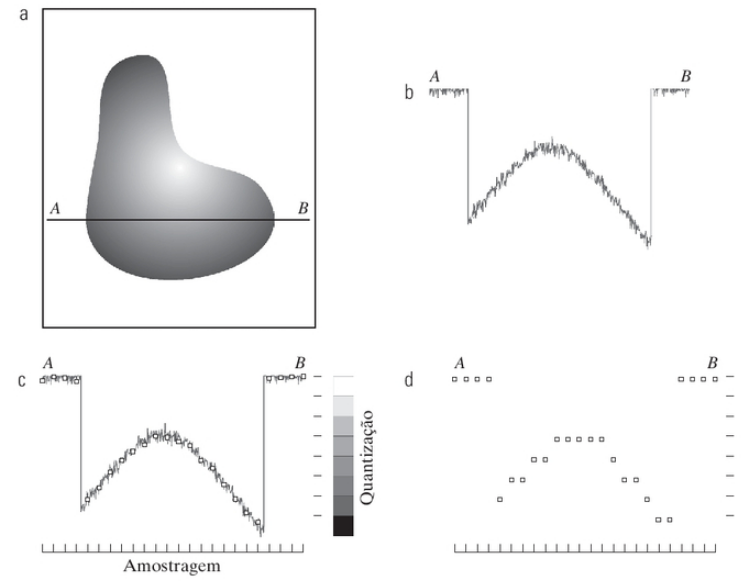
\includegraphics[width=8cm, height=8cm]{figura1}
	\captionof{figure}[]{Produzindo uma imagem digital. (a) Imagem contínua. (b) Linha de varedura de A a B na imagem contínua utilizada para ilustrar os conceitos de amostragem e quantização. (c) Amostragem e quantização. (d) Linha de varredura digital.}
	\label{medium}
\end{Figure}
A função unidimensional da Figura 1(b) é gráfico que representa os valores amplitude (nível de intensidade) da imagem contínua ao longo do segmento da reta AB na Figura 1(a). Para realizar a amostragem, colhemos amostras igualmente espaçadas ao longo da linha AB, como mostra a Figura 1(c). As amostras são representadas por pequenos quadrados brancos superpostos na função. Para formar uma imagem digital, os valores de intensidade também devem ser convertidos (quantizados) em quantidades discretas. Ao lado da Figura 1(c) mostra a escala da intensidade dividida em oito intervalos discretos, cariando do preto ao branco. Os níveis de intensidade contínuos são quantizados atribuindo um dos oitos valores para cada amostra. As amostras digitais resultantes da amostragem e quantização são mostradas na Figura 1(d). Ao começar na parte superior da imagem e realizar esse procedimento linha por linha, produz-se uma imagem digital bidimensional. Está implícito na Figura 1 que, além do número discreto de níveis utilizados, a precisão atingida depende do conteúdo de ruído do sinal da amostragem.
\par
Quando sensores por varredura de linha são utilizados para aquisição de imagem, o número de sensores da linha define as limitações da amostragem. A quantização das saídas do sensor completa o processo de formação de uma imagem digital.
\par 
Quando uma matriz de sensores é utilizada para a aquisição de uma imagem, não há movimento, e o número de sensores na matriz determina os limites da amostragem. A Figura 2 ilustra esse conceito. A Figura 2(a) mostra uma imagem contínua projetada sobre o plano de uma matriz de sensores. A Figura 2(b) mostra a imagem após a amostragem e quantização.
\begin{Figure}
	\centering 
	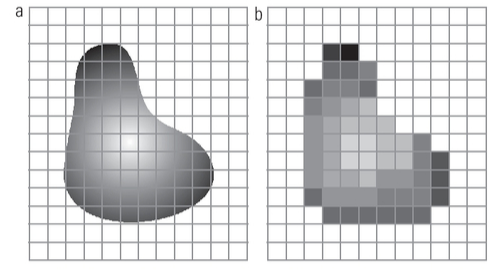
\includegraphics[width=8cm, height=5cm]{figura2}
	\captionof{figure}[]{(a) Imagem contínua projetada em uma matriz de sensores. (b) Resultado da amostragem e quantização da imagem.}
	\label{medium}
\end{Figure}

\subsection{Exemplos}
\subsubsection{Cameraman}
A amostragem está diretamente ligada com a quantidade de informação que se deseja guardar. Quanto maior a amostragem, mais detalhes teremos.
Vamos citar o exemplo do cameraman, sua representação original pode ser visualizada na Figura 3.
\begin{Figure}
	\centering 
	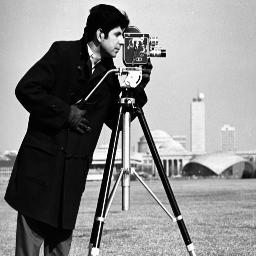
\includegraphics[width=8cm, height=8cm]{figura3}
	\captionof{figure}[]{Figura original do cameraman.}
	\label{medium}
\end{Figure}
Para execução da amostragem sobre uma imagem real, faz-se necessário definirmos uma grade de amostragem, essa grade é aplicada sobre a imagem de forma que cada célula da grande contem uma sub-imagem, conforme mostrado na Figura 4
\begin{Figure}
	\centering 
	
\includegraphics[width=8cm, height=8cm]{figura4}
	\captionof{figure}[]{Grande de amostragem.}
	\label{medium}
\end{Figure}
A Grade de Amostragem deve ser aplicada sobre a imagem original, como mostrado na Figura 5
\begin{Figure}
	\centering 
	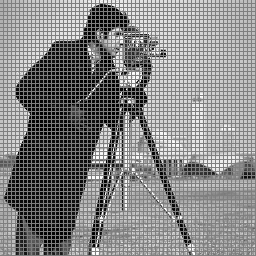
\includegraphics[width=8cm, height=8cm]{figura5}
	\captionof{figure}[]{Figura do cameraman com a Grade de Amostragem aplicada.}
	\label{medium}
\end{Figure}

Agora, vamos aplicar a Quantização escolhendo a cor dentro da imagem, levando em conta cada uma das cores de uma sub-imagem e escolhendo uma, como demonstrado na Figura 6.

\begin{Figure}
	\centering 
	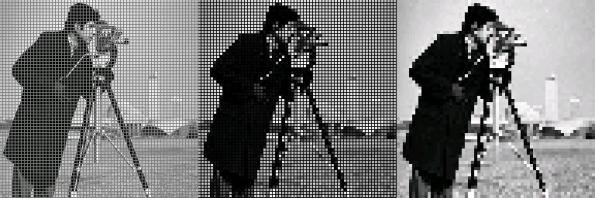
\includegraphics[width=8cm, height=3cm]{Figura6}
	\captionof{figure}[]{Processo de quantização aplicada à figura do cameraman.}
	\label{medium}
\end{Figure}
Na Figura 6(a) temos a imagem original com a grade de amostragem aplicada, na Figura 6(b) temos a imagem quantizada, e ainda com a grade de amostragem. Retirando a grade temos a Figura 6(c) final após os processos de amostragem e quantização.

\end{multicols}
\end{document}

